\chapter{曲面积分}

本章讨论第一类曲面积分和第二类曲面积分。

“第一类曲面积分”是数量值函数对曲面的积分,表示对曲面的累积量。
“第二类曲面积分”是向量值函数对曲面的积分,是两个矢量的内积。

本章要点:
\begin{itemize}
    \item 第一类曲面积分。
    \item 第二类曲面积分。
\end{itemize}

~

\newpage
\section{第一类曲线积分}

本节讨论第一类曲面积分。
所谓“第一类曲面积分”是数量值函数对曲面的积分。

本节要点:
\begin{itemize}
    \item 掌握第一类曲面积分的概念;
    \item 掌握第一类曲面积分的计算,重点掌握曲面微元的计算。
\end{itemize}

%============================================================
\subsection{第一类曲面积分的概念}

\begin{definition}[第一类曲面积分]
若三维空间中有曲面$S$,$f\left( \boldsymbol{p} \right) ,\boldsymbol{p}\in \mathbb{R} ^3$为定义在该空间上的三元数量值函数,若下式极限存在,则称极限值为{\bf $f\left( \boldsymbol{p} \right) $在$S$上积分称为第一类曲面积分},记为$\iint_S{f\left( \boldsymbol{p} \right) ds}$,即:
\[
\iint\limits_S{f\left( \boldsymbol{p} \right) ds}:=\underset{\lambda \rightarrow 0}{\lim}\sum_{i=1}^n{\left[ f\left( \xi _i,\eta _i,\zeta _i \right) \cdot \Delta s_i \right]}
\]
其中:
\begin{itemize}
    \item $f\left( \boldsymbol{p} \right) $:{\bf 被积函数};
    \item $ds$:{\bf 曲面微元};
    \item $S$:{\bf 积分曲面}。
\end{itemize}
\end{definition}

\begin{tcolorbox}
实际定义参考“教材\cite{book1}”,这里是一个简写,总体来讲就是将曲面分片,每片上取一个值和这一小片面积乘积$f\left( \xi _i,\eta _i,\zeta _i \right) \cdot \Delta s_i$,如果和式有极限,则成为$f\left( \boldsymbol{p} \right) $在$S$上有第一类曲面积分。
大致思路和一元函数积分一样。
\end{tcolorbox}

简单说明曲面微元$ds$和{\it xOy}平面投影微元$d\sigma $的关系,这是求解第一类曲面积分的关键。
如果曲面在被积范围内可微,则某点处的曲面微元$ds$与该点处的切面微元$dA$的面积相等。
若曲面由$z=z\left( x,y \right) $显式给出,则切面的法向量为$\boldsymbol{n}=\left( -z_x\,\,-z_y\,\,1 \right) ^T$。
假设法向量和{\it z}轴成角$\theta $,则有:
\[
\cos \theta =\frac{1}{\sqrt{\left( z_x \right) ^2+\left( z_y \right) ^2+1}}
\]
则切面微元$dA$和{\it xOy}平面投影微元$d\sigma $有关系:
\[
d\sigma =\cos \theta \cdot dA=\frac{1}{\sqrt{\left( z_x \right) ^2+\left( z_y \right) ^2+1}}\cdot dA
\]
可得曲面微元$ds$和{\it xOy}平面投影微元$d\sigma $的关系:
\[
ds=\sqrt{\left( z_x \right) ^2+\left( z_y \right) ^2+1}\cdot d\sigma =\sqrt{\left( z_x \right) ^2+\left( z_y \right) ^2+1}\cdot dxdy
\]

\begin{figure}[h]
\centering
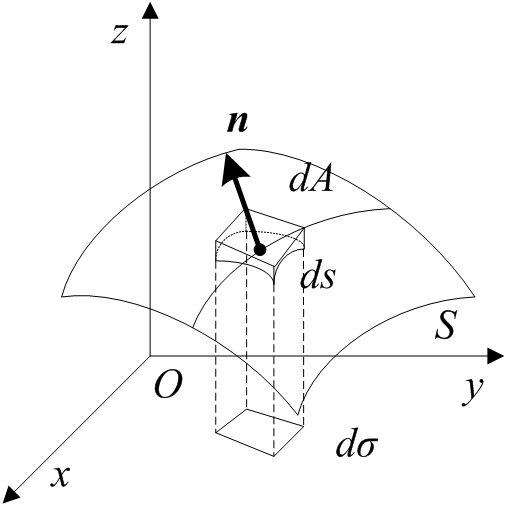
\includegraphics[height=4cm]{10.1.png}
\end{figure}

%============================================================
\subsection{第一类曲面积分的计算}

\begin{theorem}[第一类曲面积分的计算公式]
若$f\left( \boldsymbol{p} \right) $在曲面$S$上连续,$z=z\left( x,y \right) $在$S$上具有一阶连续偏导,则第一类曲面积分的计算公式有:
\begin{align*}
&\iint\limits_S{f\left( \boldsymbol{p} \right) ds}=\iint\limits_D{\left[ f\left( x,y,z\left( x,y \right) \right) \cdot \sqrt{\left( z_x \right) ^2+\left( z_y \right) ^2+1} \right] dxdy} \\
&S=\left\{ \left( x,y,z \right) \middle| x_1\leqslant x\leqslant x_2,y_1\left( x \right) \leqslant y\leqslant y_2\left( x \right) ,z=z\left( x,y \right) \right\} \\
&D=\left\{ \left( x,y \right) \middle| x_1\leqslant x\leqslant x_2,y_1\left( x \right) \leqslant y\leqslant y_2\left( x \right) \right\}
\end{align*}
\end{theorem}

第一类曲面积分的计算关键在于理解曲面微元和投影微元的关系:
\[
ds=\sqrt{\left( z_x \right) ^2+\left( z_y \right) ^2+1}\cdot d\sigma =\sqrt{\left( z_x \right) ^2+\left( z_y \right) ^2+1}\cdot dxdy
\]
通过这个关系,将第一类曲面积分化为二重积分。






\newpage
\section{第二类曲面积分}

本节讨论第二类曲面积分。
所谓“第二类曲面积分”是向量值函数对曲面的积分。

本节要点:
\begin{itemize}
    \item 掌握第二类曲面积分的概念;
    \item 掌握第二类曲面积分的计算,重点掌握积分表达式的内积计算。
\end{itemize}

%============================================================
\subsection{第二类曲面积分的概念}

\begin{definition}[第二类曲面积分]
若三维空间中有曲线$S$,$\mathbf{n}\left( \boldsymbol{p} \right) $为曲面上任一点处的单位法向量,$\boldsymbol{f}\left( \boldsymbol{p} \right) $为定义在该空间上的三元向量值函数,若内积$\boldsymbol{f}\left( \boldsymbol{p} \right) ^T\mathbf{n}\left( \boldsymbol{p} \right) $在$S$上的第一类曲面积分存在,则称此积分值为{\bf $\boldsymbol{f}\left( \boldsymbol{p} \right) $在$S$上的第二类曲面积分},记为$\iint_S{\left[ \boldsymbol{f}\left( \boldsymbol{p} \right) ^T\mathbf{n}\left( \boldsymbol{p} \right) \right] \cdot ds}$,由于$\mathbf{n}\left( \boldsymbol{p} \right) ds=\boldsymbol{ds}$为曲面微元在三个坐标平面的投影,所以更普遍地记作$\iint_S{\boldsymbol{f}\left( \boldsymbol{p} \right) ^T\boldsymbol{ds}}$,即:
\begin{align*}
&\iint\limits_S{\left[ \boldsymbol{f}\left( \boldsymbol{p} \right) ^T\mathbf{n}\left( \boldsymbol{p} \right) \right] \cdot ds}=\iint\limits_S{\boldsymbol{f}\left( \boldsymbol{p} \right) ^T\boldsymbol{ds}} \\
&:=\underset{\lambda \rightarrow 0}{\lim}\sum_{i=1}^n{\left[ \boldsymbol{f}\left( \xi _i,\eta _i,\zeta _i \right) ^T\mathbf{n}\left( \xi _i,\eta _i,\zeta _i \right) \cdot \Delta s_i \right]}
\end{align*}
其中:
\begin{itemize}
    \item $\boldsymbol{f}\left( \boldsymbol{p} \right) $:{\bf 被积函数};
    \item $\mathbf{n}\left( \boldsymbol{p} \right) $:曲面$S$的{\bf 单位法向量};
    \item $\boldsymbol{ds}=\mathbf{n}\left( \boldsymbol{p} \right) ds$:{\bf 有向曲面微元};
    \item $S$:{\bf 积分曲面}。
\end{itemize}
特别地,当$S$为封闭曲面时,记为$\oiint_S{\boldsymbol{f}\left( \boldsymbol{p} \right) ^T\boldsymbol{ds}}$。
\end{definition}

这里要注意,第二类曲面积分是有方向性的,默认方向是曲面的法方向,如果取反方向,则写为:
\[
\iint\limits_{S^-}{\boldsymbol{f}\left( \boldsymbol{p} \right) ^T\boldsymbol{ds}}
\]

%============================================================
\subsection{第二类曲面积分的计算}

\begin{theorem}[第二类曲面积分的计算公式]
我们知道有向曲面微元有:
\begin{align*}
\boldsymbol{ds}&=\mathbf{n}\left( \boldsymbol{p} \right) ds=\frac{\left( -z_x\,\,-z_y\,\,1 \right) ^T}{\sqrt{\left( z_x \right) ^2+\left( z_y \right) ^2+1}} \left[ \sqrt{\left( z_x \right) ^2+\left( z_y \right) ^2+1}\cdot dxdy \right] \\
&=\left( \begin{array}{c}
	-z_x\\
	-z_y\\
	1\\
\end{array} \right) dxdy
\end{align*}
所以向量值函数$\boldsymbol{f}\left( \boldsymbol{p} \right) =\left( P\,\,Q\,\,R \right) ^T$的第二类曲面积分的计算有:
\begin{align*}
\iint\limits_S{\boldsymbol{f}\left( \boldsymbol{p} \right) ^T\boldsymbol{ds}}&=\iint\limits_S{\left( \begin{array}{c}
	P\\
	Q\\
	R\\
\end{array} \right) ^T\left( \begin{array}{c}
	-z_x\\
	-z_y\\
	1\\
\end{array} \right) dxdy} \\
&=\iint\limits_S{\left( -Pz_x-Qz_y+R \right) dxdy}
\end{align*}
\end{theorem}

这里,第二类曲面积分的计算是将有向曲面微元投影到{\it xOy}平面,也可以投影到其他平面,看曲面以什么形式给出。
和第二类曲线积分一样,重点理解被积表达式中的内积。

曲面$S$的单位法向量可写成方向余弦形式$\mathbf{n}=\left( \cos \alpha \,\,\cos \beta \,\,\cos \gamma \right) ^T$,于是积分:
\[
\iint\limits_S{\boldsymbol{f}\left( \boldsymbol{p} \right) ^T\boldsymbol{ds}}=\iint\limits_S{\left( \begin{array}{c}
	P\\
	Q\\
	R\\
\end{array} \right) ^T\left( \begin{array}{c}
	\cos \alpha\\
	\cos \beta\\
	\cos \gamma\\
\end{array} \right) ds}
\]
而又有投影关系:
\begin{align*}
&\cos \alpha \cdot ds=dydz \\
&\cos \beta \cdot ds=dzdx \\
&\cos \gamma \cdot ds=dxdy
\end{align*}
所以第二类曲面积分还可以写为:
\[
\iint\limits_S{\boldsymbol{f}\left( \boldsymbol{p} \right) ^T\boldsymbol{ds}}=\iint\limits_S{Pdydz+Qdzdx+Rdxdy}
\]
这表明$\boldsymbol{f}\left( \boldsymbol{p} \right) $在$S$上的积分可以分解为其三个坐标分量($P,Q,R$)分别对坐标平面({\it yOz}、{\it zOx}和{\it xOy})积分的代数和。






\newpage
\section{两类曲面积分的对比和意义}

本节首先对比两类曲面积分,分析它们的区别,再讨论它们的物理意义。

本节要点:
\begin{itemize}
    \item 理解“对曲面”和“对坐标平面”的含义;
    \item 理解曲面积分的物理意义。
\end{itemize}

%============================================================
\subsection{曲面积分的对比}

将三重积分和两类曲面积分放在一起,
\begin{align*}
&\iiint\limits_V{f\left( \boldsymbol{p} \right) dv} \\
&\iint\limits_S{f\left( \boldsymbol{p} \right) ds} \\
&\iint\limits_S{\boldsymbol{f}\left( \boldsymbol{p} \right) ^T\mathbf{n}\left( \boldsymbol{p} \right) \cdot ds}=\iint\limits_S{\boldsymbol{f}\left( \boldsymbol{p} \right) ^T\boldsymbol{ds}}
\end{align*}
可以看到:
\begin{itemize}
    \item 第一类曲面积分和三重积分的区别只在积分区域,前者是曲面,后者是三维体;
    \item 第一类曲面积分的积分区域是一个曲面,所以又称{\bf 对曲面面积的积分};
    \item 第二类曲面积分又可以写成坐标平面分量的形式,所以又称{\bf 对坐标平面的曲面积分};
    \item 两种曲面积分的区别在于被积函数,第二类曲面积分的被积函数是向量值函数在切面法方向上的投影$\boldsymbol{f}\left( \boldsymbol{p} \right) ^T\mathbf{n}\left( \boldsymbol{p} \right) $,或者说第二类曲面积分的积分表达式是两个向量函数的内积$\boldsymbol{f}\left( \boldsymbol{p} \right) ^T\boldsymbol{ds}$;
    \item 计算方法上,都是化成重积分求解。
\end{itemize}

\begin{tcolorbox}
从式子上看,只要看到$ds$的都是第一类曲面积分,有$dxdy,dydz,dzdx$单独出现的就是第二类曲面积分。
\end{tcolorbox}

%============================================================
\subsection{曲面积分的物理意义}

物理上,第一类曲面积分表示一数量场对曲面的总量,如弧面的质量、非均匀带电球面的电荷总量等。
第二类曲面积分是计算一矢量场对曲面的总通量的问题,如果是电场,则通量就是通过该曲面的电通量,如果是水流,则通量就是流过该曲面的水流量。

举例说明,三维空间中,一个固定方向的流速均匀流速场通过一个垂直平面的流量为$v\cdot S$。
如果平面和流速场方向不一致,则需要引入它们之间的夹角$v\cdot S\cdot \cos \theta $,可以理解为平面在流速场方向的投影,也可以理解为两个矢量的内积$\boldsymbol{v}^T\boldsymbol{S}$。

\begin{figure}[h]
\centering
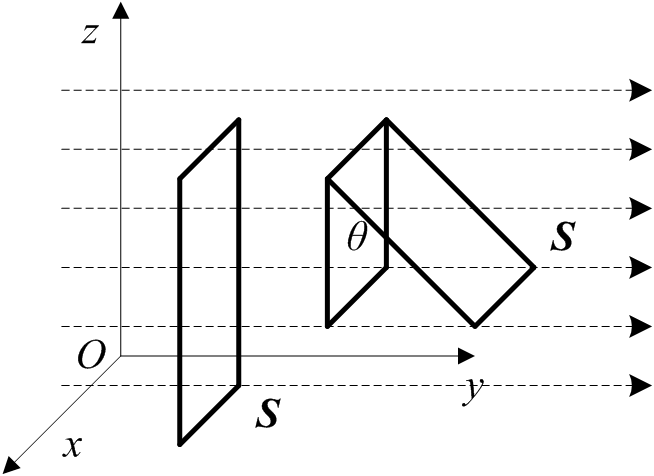
\includegraphics[height=3.5cm]{10.2.png}
\end{figure}

%============================================================
\subsection{计算方法对比}

假设曲面$S=\left\{ \left( x,y,z \right) |x_1\leqslant x\leqslant x_2,y_1\left( x \right) \leqslant y\leqslant y_2\left( x \right) ,z=z\left( x,y \right) \right\} $。
根据给出的曲面方程,投影到{\it xOy}平面。

第一类曲面积分:
\begin{align*}
&\iint\limits_S{f\left( \boldsymbol{p} \right) ds} \qquad ds=\sqrt{\left( z_x \right) ^2+\left( z_y \right) ^2+1}\cdot dxdy \\
&\Downarrow \\
&\iint\limits_S{f\left( \boldsymbol{p} \right) ds}=\iint\limits_D{\left[ f\left( x,y \right) \cdot \sqrt{\left( z_x \right) ^2+\left( z_y \right) ^2+1} \right] dxdy} \\
&D=\left\{ \left( x,y \right) \middle| x_1\leqslant x\leqslant x_2,y_1\left( x \right) \leqslant y\leqslant y_2\left( x \right) \right\}
\end{align*}

第二类曲面积分:
\begin{align*}
&\iint\limits_S{\boldsymbol{f}\left( \boldsymbol{p} \right) ^T\boldsymbol{ds}} \qquad \boldsymbol{ds}=\mathbf{n}\left( \boldsymbol{p} \right) ds=\left( -z_x\,\,-z_y\,\,1 \right) ^Tdxdy \\
&\Downarrow \\
&\iint\limits_S{\boldsymbol{f}\left( \boldsymbol{p} \right) ^T\boldsymbol{ds}}=\iint\limits_S{\left[ -P\left( x,y \right) \cdot z_x-Q\left( x,y \right) \cdot z_y+R\left( x,y \right) \right] dxdy} \\
&D=\left\{ \left( x,y \right) \middle| x_1\leqslant x\leqslant x_2,y_1\left( x \right) \leqslant y\leqslant y_2\left( x \right) \right\}
\end{align*}






\newpage
\section{多元积分总结}

由于多元能产生矢量,所以多元积分分数量值积分和向量值积分,但无论哪个积分,最终结果都是一个标量值。

数量值积分的被积函数是数量值函数,表示数量值对于被积区域的累积,可分为重积分、线积分、面积分,向量值积分的被积函数是向量值函数,表示向量值在有向被积区域内的累积,可分为线积分和面积分。

对于数量值函数:
\begin{table}[h]
\centering
\begin{tabular}{lll}
    \toprule
    名称 & 表达式 & 物理意义\\
    \midrule
    重积分   & $\iiint_V{f\left( \boldsymbol{p} \right) dv}$ & 体质量\\
    曲线积分 & $\int_L{f\left( \boldsymbol{p} \right) dl}$   & 曲线质量\\
    曲面积分 & $\iint_S{f\left( \boldsymbol{p} \right) ds}$  & 曲面质量\\
    \bottomrule
\end{tabular}
\end{table}

对于向量值函数:
\begin{table}[h]
\centering
\begin{tabular}{lll}
    \toprule
    名称 & 表达式 & 物理意义\\
    \midrule
    曲线积分 & $\int_L{\boldsymbol{f}\left( \boldsymbol{p} \right) ^T\boldsymbol{dl}}$  & 矢量场的环流量\\
    曲面积分 & $\iint_S{\boldsymbol{f}\left( \boldsymbol{p} \right) ^T\boldsymbol{ds}}$ & 矢量场的通量\\
    \bottomrule
\end{tabular}
\end{table}






\newpage
\section{习题}

\begin{exercise}
已知球面$x^2+y^2+z^2=R^2$,求包含在柱面$x^2+y^2=Rx$中的部分的面积。
\end{exercise}

解:

基本思路是求解一个区域内曲面的面积。
由于对称性,只计算第一卦限。
首先分析积分区域,得:
\[
S=\left\{ \left( x,y,z \right) \middle| 0\leqslant x\leqslant R,0\leqslant y\leqslant \sqrt{Rx-x^2},z=\sqrt{R^2-x^2-y^2} \right\}
\]
于是面积:
\begin{align*}
&A=4\iint\limits_S{ds}=4\iint\limits_D{\sqrt{1+{z_x}^2+{z_y}^2}dxdy}=4R\iint\limits_D{\frac{1}{\sqrt{R^2-x^2-y^2}}dxdy} \\
&D=\left\{ \left( x,y \right) \middle| 0\leqslant x\leqslant R,0\leqslant y\leqslant \sqrt{Rx-x^2} \right\}
\end{align*}
为计算简单,化为极坐标:
\begin{align*}
&A=4R\iint\limits_D{\frac{r}{\sqrt{R^2-r^2}}drd\theta} \\
&D=\left\{ \left( r,\theta \right) \middle| 0\leqslant \theta \leqslant \frac{\pi}{2},0\leqslant r\leqslant R\cos \theta \right\}
\end{align*}
解得:
\begin{align*}
A&=4R\int_0^{\frac{\pi}{2}}{d\theta \int_0^{R\cos \theta}{\frac{r}{\sqrt{R^2-r^2}}dr}} \\
&=4R\int_0^{\frac{\pi}{2}}{\left( R-R\sin \theta \right) d\theta}=\left( 2\pi -4 \right) R^2
\end{align*}


~

\begin{exercise}
设有流速场$\boldsymbol{v}\left( \boldsymbol{p} \right) =\left( x\,\,y\,\,z \right) $,求通过曲面$S:x^2+y^2+z^2=R^2,z\geqslant 0$的流量。
\end{exercise}

解:

曲面是一个位于原点的球形的上半部分。
大致思路就是构建第二类曲面积分方程,主要是被积函数和积分曲面,然后求解。

首先构建积分方程:
\[
\varPhi =\iint\limits_S{\boldsymbol{v}^T\boldsymbol{ds}}=\iint\limits_S{\left( \begin{array}{c}
	x\\
	y\\
	z\\
\end{array} \right) ^T\left( \begin{array}{c}
	-z_x\\
	-z_y\\
	1\\
\end{array} \right) dxdy}=\iint\limits_S{\left( -xz_x-yz_y+z \right) dxdy}
\]
求解$z_x,z_y$,需要用到隐函数偏导方法,构建隐函数$F\left( x,y,z \right) =x^2+y^2+z^2-R^2$:
\begin{align*}
&z_x=-\frac{F_x}{F_z}=-\frac{x}{z} \\
&z_y=-\frac{F_y}{F_z}=-\frac{y}{z}
\end{align*}
代入得:
\begin{align*}
&\varPhi =\iint\limits_S{\left( \frac{x^2}{z}+\frac{y^2}{z}+z \right) dxdy}=\iint\limits_S{\frac{R^2}{z}dxdy}=\iint\limits_D{\frac{R^2}{\sqrt{R^2-x^2-y^2}}dxdy} \\
&D=\left\{ \left( x,y \right) \middle| -R\leqslant x\leqslant R,-\sqrt{R^2-x^2}\leqslant y\leqslant \sqrt{R^2-x^2} \right\}
\end{align*}
转换到极坐标求解:
\begin{align*}
\varPhi &=\iint\limits_D{\frac{R^2}{\sqrt{R^2-r^2}}rdrd\theta}=R^2\int_0^{2\pi}{d\theta \int_0^R{\frac{r}{\sqrt{R^2-r^2}}dr}} \\
&=R^2\int_0^{2\pi}{Rd\theta}=2\pi R^3
\end{align*}









